\documentclass[a4paper,12pt, notitlepage]{report}
\usepackage[margin=2.5cm]{geometry}
\usepackage{listings}
\usepackage[parfill]{parskip}
\setlength{\parskip}{\baselineskip}%
\setlength{\parindent}{0pt}%
\usepackage{amsmath}
\usepackage{amssymb}
\usepackage{graphicx}
\usepackage[justification=centering]{caption}
\usepackage{epstopdf}
\usepackage[usenames, dvipsnames]{color}
\usepackage{chngcntr}
\usepackage{titling}
%\counterwithout{footnote}{chapter}
\usepackage{float}
%\renewcommand\theContinuedFloat{\alph{ContinuedFloat}}
\newcommand\tab[1][0.05cm]{\hspace*{#1}}

\title{Numerical Assignment}
\author{Mariana Clare}
\date{\today}

\begin{document}
	
\maketitle
\thispagestyle{empty}
\section*{Defining Shallow Water Equations}
The shallow water equations are
\begin{equation}\label{momentumsw}
\frac{\partial \mathbf{u}}{\partial t} + \mathbf{u}\cdot\nabla\mathbf{u} = - 2\Omega \times\mathbf{u} - g\nabla (h + h_{0})
\end{equation}
\begin{equation}\label{masssw}
\frac{\partial h}{\partial t} + \mathbf{u}\cdot\nabla h = - h \nabla \cdot \mathbf{u}
\end{equation}
where $\mathbf{u}$ is the velocity of the flow, $\Omega$ is the angular velocity of the rotating frame of reference, $g$ is the gravitational acceleration constant, $h$ is the depth of the fluid and $h_{0}$ represents the underlying shape that the fluid is flowing over (as defined in \cite{MPE textbook}).

The first equation (\ref{momentumsw}) represents the conservation of momentum and the second equation (\ref{masssw}) represents the conservation of mass. Both equations have a $u\cdot\nabla$ which represents advection.

In order to solve these equations numerically, they first need to be linearised about the state $u = 0$ and $h = H$ ie.
\begin{eqnarray}\nonumber
\mathbf{u} =  & \mathbf{\hat{u}}
 \\   \nonumber
h = &  H + \hat{h} .
\end{eqnarray}
where $H$ is the average fluid depth. If we further assume that $h_{0}$ is constant, this gives
\begin{equation}
\frac{\partial \mathbf{\hat{u}}}{\partial t} = 2 \Omega \times \mathbf{\hat{u}} - g \nabla \hat{h}
\end{equation}
\begin{equation}
\frac{\partial \hat{h}}{\partial t} = - H \nabla \cdot \mathbf{\hat{u}}
\end{equation}

These equations can be simplified further by assuming there is no rotation and taking the one-dimensional form. Dropping the $\hat{}$ notation this gives
\begin{equation}\label{linearisedsw1}
\frac{\partial u}{\partial t} = - g \frac{\partial h}{\partial x}
\end{equation}
\begin{equation}\label{linearisedsw2}
\frac{\partial h}{\partial t} = - H \frac{\partial u}{\partial x}.
\end{equation}
This report will seek to solve these one-dimensional lineriased shallow water equations numerically.

\section*{Numerical Methods}

The first numerical method we use to attempt to solve (\ref{linearisedsw1}) and (\ref{linearisedsw2}) is a simple colocated forward-backward in time and centred in space scheme. As in \cite{MPE textbook}, we consider the scheme to be forward in $u$ and backward in $h$. Co-located means we define the velocity and the height at the same location in space on the meshgrid and these schemes are also referred to as A-grid or unstaggered schemes.

This scheme can be written as 
\begin{equation} \label{FTCSAgrid}
\frac{u_{j}^{(n+1)} - u_{j}^{(n)}}{\Delta t} = -g \frac{h_{j+1}^{(n)} - h_{j-1}^{(n)}}{2\Delta x}
\end{equation}
\begin{equation}\label{BTCSAgrid}
\frac{h_{j}^{(n+1)} - h_{j}^{(n)}}{\Delta t} = -H \frac{u_{j+1}^{(n+1)} - u_{j-1}^{(n+1)}}{2\Delta x}
\end{equation}
where $h_{j}^{(n)} = h(x_{j}, t^{(n)})$, $u_{j}^{(n)} = h(u_{j}, t^{(n)})$, $x_{j} = j\Delta x$ and $t^{(n)} = n\Delta t$. 

We can determine the order of accuracy of this scheme, by using Taylor series. We note the following Taylor series expansions:

\begin{equation}\label{ujn+1}
u_{j}^{(n+ 1)} = u_{j}^{(n)} + \Delta t \frac{\partial u_{j}^{(n)}}{\partial t} + \frac{(\Delta t)^{2}}{2}\frac{\partial^{2} u_{j}^{(n)}}{\partial t^{2}} + O((\Delta t)^{3})
\end{equation}
\begin{equation}\label{hj+-1n}
h_{j \pm 1}^{(n)} = h_{j}^{(n)} \pm \Delta x  \frac{\partial h_{j}^{(n)}}{\partial x} + \frac{(\Delta x)^{2}}{2}\frac{\partial^{2} h_{j}^{(n)}}{\partial x^{2}} \pm \frac{(\Delta x)^{3}}{6}\frac{\partial^{3} h_{j}^{(n)}}{\partial x^{3}} + O((\Delta x)^{4})
\end{equation}

Substuting these expansions into the scheme (\ref{FTCSAgrid}), we find that 

\begin{equation}
\frac{\partial u_{j}^{(n)}}{\partial t} + O(\Delta t) =  -g \frac{\partial h_{j}^{(n)}}{\partial x} + O((\Delta x)^{2})
\end{equation} 
and therefore the scheme is first order accurate in time and second order accurate in space. (Note the same order of accuracy is obtained by performing the same analysis with (\ref{BTCSAgrid})).

In order to find when this scheme is stable, we use a von-neumann stability analysis. As in \cite{MPE textbook}, we assume that $u$ and $h$ have wave-like solutions with an amplification factor $A$ and wavenumber $k$:
\begin{equation} \label{wavelikeu}
u  =  \mathbb{U}  A^{n} e^{ikj\Delta x}
\end{equation}
\begin{equation} \label{wavelikeh}
h  =  \mathbb{H} A^{n} e^{ikj\Delta x}
\end{equation}
for constant $\mathbb{U}$ and $\mathbb{H}$.

Further if we define the courant number 
\begin{equation}\label{courantnumber}
c = \frac{\sqrt{gH}\Delta t}{\Delta x}
\end{equation}

then substituting these solutions into (\ref{FTCSAgrid}) and (\ref{BTCSAgrid}) gives
\begin{equation}
A = 1 - \frac{c^{2}}{2} \sin^{2}(k\Delta x) \pm \frac{ic}{2}\sin(k\Delta x)\sqrt{4 - c^{2}\sin^{2}k\Delta x}.
\end{equation} 
 
Hence as found in \cite{MPE textbook}, when $\lvert c \rvert \leq 2$, $\lvert A \rvert^{2} = 1$ and the scheme is stable, but when $\lvert c \rvert > 2$, the scheme is unstable.
 
We can also find the dispersion relation, because the frequency of the numerical method is 
\begin{equation} \label{frequency}
\omega = \pm \frac{1}{\Delta t} \arctan\bigg(\frac{Im(A)}{Re(A)}\bigg)
\end{equation}
Using the result from \cite{MPE textbook}, 
\begin{equation}
\omega_{n}\Delta x = \pm \frac{2}{c} \sin^{-1} \bigg(\frac{c}{2}\sin(k\Delta x)\bigg)
\end{equation}
assuming $\sqrt{gH} = 1$. The positive branch of this dispersion relation is plotted in Figure \ref{dispersionfigure} and compared with the dispersion relation of the analytical solution. (The dispersion relation of the analytical solution $\omega = k\sqrt{gH}$ is found by substituting the wave-like solutions (\ref{wavelikeu}) and (\ref{wavelikeh}) into (\ref{linearisedsw1}) and (\ref{linearisedsw2})).


However, we would like to have a method that was stable for all courant numbers. Therefore another method we can use is an implicit method on a colocated grid. As in \cite{MPE textbook}, we look at the forward in time for both $u$ and $h$ and centred in space colocated scheme:
\begin{equation} \label{FTimplicitAgrid1}
\frac{u_{j}^{(n+1)} - u_{j}^{(n)}}{\Delta t} = -g \frac{h_{j+1}^{(n+1)} - h_{j-1}^{(n+1)}}{2\Delta x}
\end{equation}
\begin{equation}\label{FTimplicitAgrid2}
\frac{h_{j}^{(n+1)} - h_{j}^{(n)}}{\Delta t} = -H \frac{u_{j+1}^{(n+1)} - u_{j-1}^{(n+1)}}{2\Delta x}.
\end{equation}

In order to find the values of $h_{j}^{n}$ and $u_{j}^{n}$ at the next time iteration for all $j$, we consider the matrix:

\[
A = \left (
\begin{array}{ccc}
\begin{array}{ccccc}
1 + \frac{c^{2}}{2} & 0 & -\frac{c^{2}}{4} & 0 & 0\\
0 & 1 + \frac{c^{2}}{2} & 0 & -\frac{c^{2}}{4} & 0\\
-\frac{c^{2}}{4}& 0 & 1 + \frac{c^{2}}{2} & 0 & -\frac{c^{2}}{4} 
\end{array}
& \cdots & 
\begin{array}{l}
a+b+c+d+e+f+g+h\\
+i+j+k+l+m+n+o 
\end{array} \\
\vdots & \ddots & \vdots\\
\begin{array}{l}
a+b+c+d+e+f+g+h\\
+i+j+k+l+m+n+o 
\end{array} &
\cdots & 
\begin{array}{ccccc}
-\frac{c^{2}}{4}& 0 & 1 + \frac{c^{2}}{2} & 0 & -\frac{c^{2}}{4} \\
0 & -\frac{c^{2}}{4} & 0 & 1 + \frac{c^{2}}{2} & 0\\
0 & 0 & -\frac{c^{2}}{4}& 0 & 1 + \frac{c^{2}}{2}
\end{array}
\end{array}
\right )
\]
where $c$ is the courant number as before. We then rewrite the scheme (\ref{FTimplicitAgrid1}) and (\ref{FTimplicitAgrid2}) as the matrix equation $A \mathbf{x} = \mathbf{b}$ where 
\begin{equation}
x_{j} = h_{j}^{(n+1)} \text { and } b_{j} = h_{j}^{(n)} - \frac{c}{2}\sqrt{\frac{H}{g}}(u_{j+1}^{(n)} - u_{j-1}^{(n)})
\end{equation}
if solving for $h$ and
\begin{equation}
x_{j} = u_{j}^{(n+1)} \text { and } b_{j} = u_{j}^{(n)} - \frac{c}{2}\sqrt{\frac{g}{H}}(h_{j+1}^{(n)} - h_{j-1}^{(n)})
\end{equation}
if solving for $u$.

Note that here and throughout this report we are assuming periodic boundary conditions and hence that $u_{0}^{(n)} = u_{N}^{(n)}$ and $h_{0}^{(n)} = h_{N}^{(n)}$

We can determine the order of accuracy of this scheme, as before by using the Taylor series expansions (\ref{ujn+1}) and
\begin{equation}
h_{j \pm 1}^{(n+1)} = h_{j}^{(n)} \pm \Delta x \frac{\partial h_{j}^{(n)}}{\partial x} + \frac{(\Delta x)^{2}}{2} \frac{\partial^{2}h_{j}^{(n)}}{\partial x^{2}} \pm \Delta x \Delta t \frac{\partial^{2}h_{j}^{(n)}}{\partial x\partial t} + \frac{(\Delta t)^{2}}{2}\frac{\partial^{2}h_{j}^{(n)}}{\partial t^{2}} + O((\Delta x)^{3}, {(\Delta t)^{3}}).
\end{equation}
Substituting this into equation (\ref{FTimplicitAgrid1}) we find that
\begin{equation}
\frac{\partial u_{j}^{(n)}}{\partial t} + O(\Delta t) = - g \frac{\partial h_{j}^{(n)}}{\partial x} + O((\Delta x)^{2}).
\end{equation}
Therefore the scheme is first order accurate in time and second order accurate in space as with the explicit method on the colocated grid. (As before a similar result can be obtained by substituting in to (\ref{FTimplicitAgrid2})).

In order to find where this method is stable, we use von-neumann stability analysis and assume $u$ and $h$ have wave-like solutions (\ref{wavelikeu}) and (\ref{wavelikeh}). Substituting these solutions into (\ref{FTimplicitAgrid1}) and (\ref{FTimplicitAgrid2}) we find
\begin{equation}
A = \frac{1 \pm i c\sin(k\Delta x)}{1 + c^{2}\sin^{2}(k\Delta x)}
\end{equation}
Therefore 
\begin{equation}
\lvert A \rvert ^{2} = \frac{1}{1 + c^{2}\sin^{2}(k\Delta x)} < 1  \tab[1cm] \forall k, \Delta x
\end{equation}
and the system is stable everywhere. 

Using (\ref{frequency}) we can find the dispersion relation
\begin{equation}
\omega_{n} \Delta x = \pm\frac{\Delta x}{\Delta t} \arctan(c\sin(k\Delta x)) = \frac{1}{c}  \arctan(c\sin(k\Delta x))
\end{equation}
assuming $\sqrt{gH} = 1$. The positive branch of this dispersion relation is again plotted in Figure \ref{dispersionfigure}.

We can see from this Figure \ref{dispersionfigure} that the analytic solution and numerical solution do not propagate at the same rate. The numeric solution disperses too slowly and in fact at $k = \pi$, the wave is stationary. 

Therefore we seek a scheme which propagates at a more similar speed to the analytic solution. Following \cite{MPE textbook}, we use a staggered grid (sometimes known as a C-grid) instead of a co-located grid. For a staggered grid, we shift $u$ so that it is defined at $x_{j} + \frac{\Delta x}{2}$ and $h$ remains defined at $x_{j}$ (where $x_{j} = j \Delta x$) ie. where $u$ and $h$ are defined alternates in space.

As in \cite{MPE textbook}, we take again the forward-backward in time and centred in space scheme where the scheme is forward in $u$ and backward in $h$, but this time on a staggered grid. This gives us the following scheme:

\begin{equation}\label{FTCSCgrid}
\frac{u_{j+ \frac{1}{2}}^{(n+1)} - u_{j + \frac{1}{2}}^{(n)}}{\Delta t} = -g \frac{h_{j+1}^{(n)} - h_{j}^{(n)}}{\Delta x}
\end{equation}

\begin{equation}\label{BTCSCgrid}
\frac{h_{j}^{(n+1)} - h_{j}^{(n)}}{\Delta t} = -H \frac{u_{j+\frac{1}{2}}^{(n+1)} - u_{j-\frac{1}{2}}^{(n+1)}}{\Delta x}
\end{equation}


We can determine the order of accuracy of this scheme, as before, by using the Taylor series expansions (\ref{hj+-1n}) and 
\begin{equation} \label{uj+1/2n}
u_{j \pm \frac{1}{2}}^{(n)} = u_{j}^{(n)} \pm \frac{\Delta x}{2}\frac{\partial u_{j}^{(n)}}{\partial x} + \frac{(\Delta x)^{2}}{8}\frac{\partial^{2}u_{j}^{n}}{\partial x^{2}} + O({(\Delta x)^{3}}.
\end{equation}
\begin{equation} \label{uj+1/2n+1}
u_{j \pm \frac{1}{2}}^{(n + 1)} = u_{j}^{(n)} \pm \frac{\Delta x}{2}\frac{\partial u_{j}^{(n)}}{\partial x} + \Delta t \frac{\partial u_{j}^{(n)}}{\partial t} + \frac{(\Delta x)^{2}}{8}\frac{\partial^{2}u_{j}^{n}}{\partial x^{2}} \pm \frac{\Delta t \Delta x}{2}\frac{\partial^{2} u_{j}^{(n)}}{\partial x \partial t} + \frac{(\Delta t)^{2}}{2} \frac{\partial ^{2} u_{j}^{(n)}}{\partial t ^{2}} + O((\Delta x)^{3}, (\Delta t)^{3})
\end{equation}

Substituting these into (\ref{FTCSCgrid}), we find that 
\begin{equation}
\frac{\partial u_{j}^{(n)}}{\partial t} + O(\Delta t) =  -g \frac{\partial h_{j}^{(n)}}{\partial x} + O((\Delta x)^{2})
\end{equation} 
and therefore the scheme is first order accurate in time and second order accurate in space. (Note as before the same order of accuracy is obtained by performing the same analysis with (\ref{BTCSCgrid})).

In order to find where this method is stable, we use von-neumann stability analysis and assume $u$ and $h$ have wave-like solutions (\ref{wavelikeu}) and (\ref{wavelikeh}). Substituting these solutions into (\ref{FTCSCgrid}) and (\ref{BTCSCgrid}) we find
\begin{equation}
A = 1 - 2c^{2}\sin^{2}\bigg(\frac{k\Delta x}{2}\bigg) \pm 2ic\sin\bigg(\frac{k\Delta x}{2}\bigg) \sqrt{1 - c^{2}\sin^{2}(\frac{k\Delta x}{2}\bigg)}
\end{equation}
Therefore if $\lvert c \rvert \leq 1$, this scheme is stable, but if $\lvert c \rvert > 1$ the scheme is unstable.

Using (\ref{frequency}) we can find the dispersion relation
\begin{equation}
	\omega_{n} \Delta x = \pm\frac{2\Delta x}{\Delta t} \arcsin\bigg(c\sin\bigg(\frac{k\Delta x}{2}\bigg)\bigg) = \frac{2}{c} \arcsin\bigg(c\sin\bigg(\frac{k\Delta x}{2}\bigg)\bigg) 
\end{equation}
assuming $\sqrt{gH} = 1$. The positive branch of this dispersion relation is again plotted in Figure \ref{dispersionfigure}. 

Although this solution is still dispersive we can see from the Figure that $\omega$ of this numeric scheme is much closer to $\omega$ of the analytic solution.

However we again have the problem that the solution is unstable. Therefore the final numerical scheme we will look at is the semi-implicit scheme on a staggered grid outlined in \cite{semi-implicit}.

The scheme used in \cite{semi-implicit} is the theta-method:

\begin{equation}
\frac{u_{j + \frac{1}{2}}^{(n + 1)} - u_{j + \frac{1}{2}}^{(n)}}{\Delta t} = -\frac{g}{\Delta x} \bigg(\theta (h_{j + 1}^{(n+ 1)} - h_{j}^{(n+ 1)}) + (1 - \theta) (h_{j + 1}^{(n)} - h_{j}^{(n)})\bigg)
\end{equation}
\begin{equation}
\frac{h_{j}^{(n + 1)} - h_{j}^{(n)}}{\Delta t} = -\frac{H}{\Delta x} \bigg(\theta (u_{j + \frac{1}{2}}^{(n+ 1)} - u_{j - \frac{1}{2}}^{(n+ 1)}) + (1 - \theta) (u_{j + \frac{1}{2}}^{(n)} - u_{j - \frac{1}{2}}^{(n)})\bigg)
\end{equation}

For simplicity we have taken $\theta = \frac{1}{2}$ and are therefore using the Crank-Nicholson method centred in space on a staggered grid:

\begin{equation}\label{semiimplicit1}
\frac{u_{j + \frac{1}{2}}^{(n + 1)} - u_{j + \frac{1}{2}}^{(n)}}{\Delta t} = -\frac{g}{2\Delta x} \bigg((h_{j + 1}^{(n+ 1)} - h_{j}^{(n+ 1)}) + (h_{j + 1}^{(n)} - h_{j}^{(n)})\bigg)
\end{equation}
\begin{equation}\label{semiimplicit2}
\frac{h_{j}^{(n + 1)} - h_{j}^{(n)}}{\Delta t} = -\frac{H}{2\Delta x} \bigg((u_{j + \frac{1}{2}}^{(n+ 1)} - u_{j - \frac{1}{2}}^{(n+ 1)}) + (u_{j + \frac{1}{2}}^{(n)} - u_{j - \frac{1}{2}}^{(n)})\bigg)
\end{equation}

In order to find the values of $h_{j}^{n}$ and $u_{j}^{n}$ at the next time iteration for all $j$, we consider the matrix:

\[
A = \left (
\begin{array}{ccc}
\begin{array}{ccc}
1 + \frac{c^{2}}{2} & -\frac{c^{2}}{4} & 0\\
-\frac{c^{2}}{4}& 1 + \frac{c^{2}}{2} & -\frac{c^{2}}{4} 
\end{array}
& \cdots & 
\begin{array}{l}
a+b+c+d+e+f+g+h\\
+i+j+k+l+m+n+o 
\end{array} \\
\vdots & \ddots & \vdots\\
\begin{array}{l}
a+b+c+d+e+f+g+h\\
+i+j+k+l+m+n+o 
\end{array} &
\cdots & 
\begin{array}{ccc}
-\frac{c^{2}}{4}& 1 + \frac{c^{2}}{2} & -\frac{c^{2}}{4} \\
0 & -\frac{c^{2}}{4} & 1 + \frac{c^{2}}{2}
\end{array}
\end{array}
\right )
\]
where $c$ is the courant number as before. 

We then rewrite the scheme (\ref{semiimplicit1}) and (\ref{semiimplicit2}) as the matrix equation $A \mathbf{x} = \mathbf{b}$ where 
\begin{equation}
x_{j} = h_{j}^{(n+1)} \text { and } b_{j} = -c\sqrt\frac{g}{H}(h_{j + 1}^{(n)} - h_{j}^{n}) + \frac{c^{2}}{4} u_{j + \frac{3}{2}}^{(n)} + (1 - \frac{c^{2}}{2})u_{j + \frac{1}{2}}^{(n)} + \frac{c^{2}}{4} u_{j - \frac{1}{2}}^{(n)}
\end{equation}
if solving for $h$ and
\begin{equation}
x_{j} = u_{j+ \frac{1}{2}}^{(n+1)} \text { and } b_{j} = -c\sqrt\frac{H}{g}(u_{j + \frac{1}{2}}^{(n)} - u_{j - \frac{1}{2}}^{n}) + \frac{c^{2}}{4} h_{j + 1}^{(n)} + (1 - \frac{c^{2}}{2})h_{j}^{(n)} + \frac{c^{2}}{4} h_{j - 1}^{(n)}
\end{equation}
if solving for $u$.

We can determine the order of accuracy of this scheme, as before by using the Taylor series expansions (\ref{uj+1/2n}) and (\ref{uj+1/2n+1}) and
\begin{equation}
h_{j}^{(n+ 1)} = h_{j}^{(n)} + \Delta t \frac{\partial h_{j}^{(n)}}{\partial t} + \frac{(\Delta t)^{2}}{2}\frac{\partial^{2} h_{j}^{(n)}}{\partial t^{2}} + O((\Delta t)^{3}).
\end{equation}

Substituting these into (\ref{semiimplicit2}) we find that
\begin{equation}
\frac{\partial h_{j}^{(n)}}{\partial t} + O((\Delta t)^{2}) = - H \frac{\partial u_{j}^{(n)}}{\partial x} + O((\Delta x)^{2}) 
\end{equation}
and therefore the scheme is second order accurate in time and second order accurate in space which is better than any of the other schemes we have looked at so far. (Note as before the same order of accuracy is obtained by performing the same analysis with (\ref{semiimplicit1})).

As before in order to find where this method is stable, we use von-neumann stability analysis and assume $u$ and $h$ have wave-like solutions (\ref{wavelikeu}) and (\ref{wavelikeh}). Substituting these solutions into (\ref{semiimplicit1}) and (\ref{semiimplicit2}) we find:

\begin{equation}
A = \frac{2 - 2c^{2}\sin^{2}(\frac{k\Delta x}{2}) \pm 4ic\sin(\frac{k\Delta x}{2})}{2 + 2 c^{2}\sin^{2}(\frac{k\Delta x}{2})}
\end{equation}

$\lvert A \rvert^{2} = 1$ and therefore the scheme is stable and undamping $\forall k$.

Using (\ref{frequency}) we can find the dispersion relation
\begin{equation}
\omega_{n} \Delta x = \pm\frac{\Delta x}{\Delta t} \arctan\bigg(\frac{2 c \sin(\frac{k\Delta x}{2})}{1 - c^{2} \sin^{2}(\frac{k\Delta x}{2})}\bigg) = \pm\frac{1}{c} \arctan\bigg(\frac{2 c \sin(\frac{k\Delta x}{2})}{1 - c^{2} \sin^{2}(\frac{k\Delta x}{2})}\bigg)
\end{equation}
assuming $\sqrt{gH} = 1$. The positive branch of this dispersion relation is again plotted in Figure \ref{dispersionfigure}. 

As with the previous staggered grid scheme, this solution is still dispersive. The dispersion relation for the semi-implicit staggered scheme diverges more from the analytic solution than the explicit staggered scheme but it is still significantly better than either of the colocated schemes. 

\begin{figure}
	\centering
	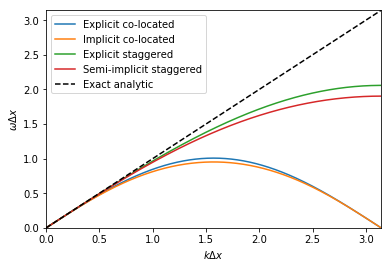
\includegraphics[width=0.7\textwidth]{dispersion_graph.png}
	\caption{Postive branch of dispersion relation $\omega$ for analytic solution and numerical schemes. Note that as in \cite{MPE textbook}, we have used $c=0.4$ and $\sqrt{gH} = 1$.} \label{dispersionfigure}
\end{figure}

\section*{Methodology to test Numerical Methods}

In order to test the properties of the Numerical methods outlined in the above section we have devised a series of tests.

To begin with, we attempt to solve the shallow water equations using a simple initial condition (shown in FIGURREEEE) with the colocated forward-backward explicit scheme.

\subsection*{Test 1}
Test to see if at courant numbers higher than 2 this colocated forward-backward explicit scheme is indeed unstable as the Von-Neumann stability analysis suggests.

\subsection* {Test 2}
Test to see if by comparison for high courant numbers the colocated forward-backward implicit scheme is in fact stable, as the Von-Neumann stability analysis suggests.

\subsection*{Test 3}
When looking at the dispersion relation for the colocated grid it seems that the results produced by the scheme may be unphysical. We test this hypothesis by taking a different initial condition (shown in FIGGURE) and plotting the solutions of $u$ and $h$ at multiple time steps for the colocated forward-backward explicit scheme.

\subsection*{Test 4}
Our analysis of the dispersion relations suggests that on a staggered grid the solutions for $u$ and $h$ should be more physical. Therefore we repeat test 3 with the same initial conditions (shown in FIGURE), but instead using the staggered explicit scheme.

\subsection*{Test 5}
So far all the comparisons have been about the properties of the schemes themselves. If the initial condition shown in FIGURE is chosen it is possible to find an analytic solution of the shallow water equations
\begin{equation}
u = \sin(x)\sin(t)
\end{equation}
\begin{equation}
h = \cos(x)\cos(t).
\end{equation}
If we choose the interval $[-\pi, \pi]$ then these solutions are periodic.

This last test will look at the error between the solutions produced by the numerical scheme and the analytic solution. It will also compare these errors to $\Delta x$ and $\Delta t$ to see if the error relationships found by the Taylor series expansions are correct.

\section*{Results}
\section*{Conclusions}

\begin{thebibliography}{9}
	\addcontentsline{toc}{part}{Bibliography}
	\bibitem{MPE textbook}
	Cotter, C. and Weller, H., (2018), \textquoteleft Numerical Methods\textquoteright, Ch.5 in Crisan, D (eds.), \textit{Mathematics of Planet Earth: a primer}, World Scientific Publishing Europe Ltd., London.
	\bibitem{semi-implicit}
	Casulli, V. and Cattani, E., (1994), \textquoteleft Stability, Accuracy and Efficiency of a Semi-Implicit Method for Three-Dimensional Shallow Water Flow\textquoteright, \textit{Computers Math. Applic}, \textbf{27(4)}, 99-112.
\end{thebibliography}
\end{document}